%!TEX root = draft.tex

\section{Attributed Random Walk Model}
\label{sec:Proposed Model}
We propose an Attributed Random Walk (\texttt{ARW}) model to explain the emergence
of key structural properties of real-world networks through \textit{entirely local}
edge formation mechanisms.

Consider a stylized example of how a researcher might go about finding relevant papers to cite. First, the researcher broadly identifies one or more \textit{relevant} papers,
possibly with the help of external information sources (e.g. Google Scholar). These initial set of papers act as seed nodes.  Then, acting under time and information constraints, she will examine papers that cite a seed paper, as well as those papers cited by the seed. Thus she navigates a chain of references to identify \textit{similar} papers relevant to addressing that research question in which she is interested. Next, through careful analysis, she will cite a subset of these papers.

\texttt{ARW} grows a directed network over time as new nodes join the network. The
mechanism is motivated by the stylized example: an incoming node selects a seed node and initiates a random walk to explore the network by navigating through neighborhoods of existing nodes. It halts the random walk after connecting to a few visited nodes.

In this section, we first describe the edge formation mechanisms underlying \texttt{ARW}. Then, we explain how \texttt{ARW} provides a unified treatment of the observations from empirical data as well as Social Science studies. Finally, we briefly discuss the methods required to fit the \texttt{ARW} model to data.


% intuitively incorporates multiple sociological phenomena.

\subsection{Model Details}
\label{sub:Model Description}


The Attributed Random Walk (\texttt{ARW}) model grows a directed network $\{\hat{G}_t\}^T_{t=1}$
in $T$ time steps.
More formally, at every discrete time step $t$, a
new node $u$, with attribute value $B(u)$, joins the network $\hat{G}_t$.
After joining the network, node $u$ forms $m(t)$ edges to
existing nodes.
% At time $t$, $G_t$ consists of ${|V_t|=|V_0|+t}$ nodes,
% ${|E_t|=|E_{t-1}|+m(t)}$ edges and the set of attribute values ${A_t = A_{t-1}
% \cup \{A(u)\}}$.
The - of incoming nodes increases over time to
reflect the nonlinear growth and densification of real networks.
% We discuss the
% issue of initializing $G_0$, sampling attribute values of inomcing nodes and modeling
% densification in \Cref{sub:Model Fitting}.

The edge formation mechanism consists of two components: \textsc{Select-Seed} and
\textsc{Random-Walk}. A new node $u$ with attribute value $B(u)$ that joins the
network at time $t$ first selects a seed node $S(u)$ using \textsc{Select-Seed}:
\\\\
\tikzstyle{background rectangle}=[thin,draw=black]
\begin{tikzpicture}[show background rectangle]
	\node[align=left, text width=.93\linewidth, inner sep=.5em]{
		(1) With probability $p_a$, randomly select $S(u)$ from the set of existing nodes that have attribute
		value $B(u)$.

		\vspace{1mm}
		(2) Otherwise, with probability $1-p_a$, randomly select $S(u)$ from the set of existing nodes that
		do \textit{not} have attribute value $B(u)$.
	};
	\node[xshift=3ex, yshift=-.7ex, overlay, fill=white, draw=white, above
	right] at (current bounding box.north west) {
		\textsc{Select-Seed}
	};
\end{tikzpicture}

% The attribute parameter $p_a$ incorporates the attribute preferences of incoming nodes
% into the model.

\textsc{Seed-Select} accounts for homophilic preferences of incoming nodes using
attribute parameter $p_a$. As shown in \cref{fig:randomwalk}, after selecting
the seed $S(u)$, node $u$ initiates a
random walk using \textsc{Random-Walk} to form $m(t)$ links.
The \textsc{Random-Walk} mechanism consists of four parameters - $\alpha$ \& $p_a$
parameterize edge formation decisions and $p_j$ \& $p_o$ characterize random walk
traversals:
\\\\
\tikzstyle{background rectangle}=[thin,draw=black]
\begin{tikzpicture}[show background rectangle]
	\node[align=left, text width=.93\linewidth, inner sep=.5em]{
		(1) At each step of the walk, new node $u$ visits node $v_i$.
		\begin{itemize}
			\item If $B(u)=B(v_i)$, $u$ links to $v_i$ with probability $\alpha \cdot p_a$
			\item Otherwise, $u$ links to $v_i$ with probability $\alpha \cdot (1-p_a)$
		\end{itemize}

		\vspace{1mm}
		(2) Then, with probability $p_j$, $u$ jumps back to seed $s_u$.

		\vspace{1mm}
		(3) Otherwise, with probability ${1-p_j}$, $u$ continues to walk. It picks an outgoing edge with probability $p_o$ \textit{or}
		an incoming edge with probability $1-p_o$ to visit a neighbor of $v_i$.

		\vspace{1mm}
		(4) Steps 1-3 are repeated until $u$ links to $m(t)$ nodes.
	};
	\node[xshift=3ex, yshift=-.7ex, overlay, fill=white, draw=white, above
	right] at (current bounding box.north west) {
		\textsc{Random-Walk}
	};
\end{tikzpicture}

When attribute data is absent, the attribute parameter $p_a$ is not required.
Then, \textsc{Seed-Select} simply selects an existing node uniformly at random
and the probability of edge formation in \textsc{Random-Walk} is equal to
the rate parameter $\alpha$ only.

Notice that \texttt{ARW} has two exogenous parameters:  the average out-degree $m(t)$ and attribute $B(u)$ of the node joining the network. The parameter $m(t)$ is similar to the parameter $m$ in the classic Preferential-Attachment model~\cite{barabasi1999emergence}, except that $m(t)$ is the mean-field value of degree $m$ at time $t$. While it is straightforward to model $m(t)$ endogenously by incoporating a densification power-law \texttt{DPL} exponent $\alpha$ to \texttt{ARW}, we decided against it, since exogenous factors to may explain changes to $m(t)$. For example, the number of citations in a paper can be influenced by venue (e.g. \texttt{WSDM2019} allows for one page of references); also, our empirical data analysis shows that papers early in a citation network tend to have few citations on average, perhaps explained by availability of \textit{fewer} papers to cite. The attribute distribution $B(u)$ varies with time as new journals or venues crop up, necessitating an exogenous parameter.



Next, we explain how each parameter is necessary to conform to normative
behavior of individuals in evolving networks.

\begin{figure*}
	\vspace{-20pt}
    \centering
    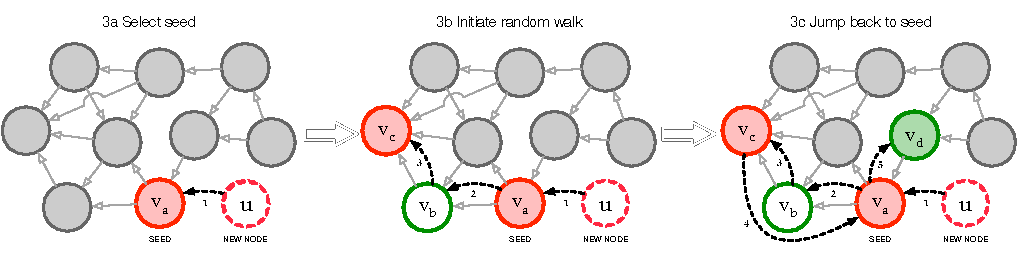
\includegraphics[width=.9\linewidth]{rw_diag}
    \caption{Edge formation in \texttt{ARW}: consider
    an incoming node $u$ with outdegree ${m=3}$ and attribute value {$B(u)=\textsc{red} \in \{\textsc{red},\textsc{green}\}$}.
    In fig. 3a, $u$ joins the network and selects seed $v_a$ via \textsc{Select-Seed}.
    Then, in fig. 3b, $u$ initiates a \textsc{Random-Walk} and traverses from $v_a$ to $v_b$ to $v_c$.
    Finally, $u$ jumps back to its seed $v_a$ and restarts the walk, as shown in fig. 3c.
    Node $u$ halts the random walk after linking to $v_a$, $v_c$ \& $v_d$.
    }
    \label{fig:randomwalk}
	\vspace{-8pt}
\end{figure*}


\subsection{\texttt{ARW} and Normative Behavior}
\label{sub:Model Interpretation}

The Attributed Random Walk model unifies multiple well-known sociological phenomena
into its edge formation mechanisms.

\newtheoremstyle{exampstyle}
  {2pt} % Space above
  {2pt} % Space below
  {\itshape} % Body font
  {} % Indent amount
  {\bfseries} % Theorem head font
  {.} % Punctuation after theorem head
  {.25em} % Space after theorem head
  {} % Theorem head spec (can be left empty, meaning `normal')

\theoremstyle{exampstyle} \newtheorem{ph}{Phenomenon}

\begin{ph}
	(Limited Resources) Individuals are boundedly rational~\cite{simon1972theories,gigerenzer1996reasoning,lipman1995information}
	actors that form edges under constraints of limited information, partial network access and finite cognitive capacity.
\end{ph}
\texttt{ARW} uses a random walk to incorporate constraints of limited information
and partial network access. A new node $u$ selects a seed node from which it
initiates a biased random walk. Then, $u$ uses simple rules to connect to each visited
nodes probabilistically and halts the walk after forming $m(t)$ edges, as shown in~\Cref{fig:randomwalk}. Random walks require information only about the
1-hop neighborhood of visited nodes, thus accounting for  the constraints of limited information and partial network access.

\begin{ph}
	(Structural Constraints) Structural factors such as network distance
	act as constraints that limit edge formation to proximate nodes.  \cite{35626}
\end{ph}

We incorporate structural constraints into \texttt{ARW} using the jump parameter $p_j$.
The jump parameter $p_j$ is the probability which a new node jumps back to its seed node
after each step of the random walk. This implies that the probability with which the new node
is at most $k$ steps from its seed node is $1-p^k_j$; As a result, the jump parameter $p_j$
controls the extent to which new nodes' random walks explore the network to form edges.

\begin{ph}
	(Triadic Closure) Nodes with common neighbors have an
	increased likelihood of forming a connection. \cite{simmel1950sociology}
\end{ph}

We control the effect of triadic closure on edge formation using the
rate parameter $\alpha$. A new node $u$ uses a random walk to
link to each visited node with probability proportional to $\alpha$. As a
result, the probability with which node $u$ closes a triad by linking to
a visited node and its neighbor is proportional to $\alpha^2$.

\begin{ph}
	(Attribute Homophily) Nodes that have similar attributes are more likely
	to form a connection. \cite{mcpherson2001birds}
\end{ph}
We incorporate attribute homophily into the edge formation process via attribute parameter $p_a$. New node
$u$ links to each visited node $v$ with probability $\alpha \cdot p_a$ if they share
the same attribute value. Otherwise, $u$ connects to $v$ with probability $\alpha \cdot (1-p_a)$.
The attribute parameter $p_a$ effectively controls the global assortativity coefficient.

\begin{ph}
	(Preferential Attachment) Nodes tend to link to high degree nodes that have more
	visibility. \cite{barabasi1999emergence}
\end{ph}
% Individuals cannot link to high degree nodes \textit{directly} under constraints of limited information
% and partial network access.
\texttt{ARW} does not use the global degree distribution. In absence of this global information, \texttt{ARW} can control the degree of preferential attachment by adding structural bias to the random walk traversals by varying the outward link probability $p_o$. Random walks that traverse outgoing edges only (i.e. $p_o =1$) eventually visit old nodes that tend to have high in-degree. Similarly, random walks that traverse incoming edges only (i.e. $p_o=0$) visit recently joined nodes that tend to have low indegree. We use parameter $p_o$, to adjust the effect of preferential attachment on edge formation.

To summarize: \texttt{ARW} accounts for five well-known sociological phenomena---bounded rationality; structural constraints; triadic closure; attribute homophily; preferential attachment---into a single edge
formation mechanism based on random walks.

% Random walks inherently account for
% limited information and partial network access. Furthermore, the jump parameter $p_j$, attribute parameter $p_a$,
% rate parameter $\alpha$ and out parameter $p_o$ incorporate the effect of structural constraints,
% homophily, triadic closure and preferential attachment respectively.



\subsection{Model Fitting}
\label{sub:Model Fitting}

We now briefly describe methods to estimate model parameters,
initialize $\hat{G}$ at time ${t=0}$, densify $\hat{G}$
over time and sample incoming nodes' attribute values.

\textit{Parameter Estimation}.
% The rate parameter $\alpha$, attribute parameter $p_a$, jump parameter $p_j$ and
% out parameter $p_o$ jointly control the edge formation mechanism in \texttt{ARW}.
% These parameters subsequently determine the structural properties of the network $\hat{G}$
% generated by \texttt{ARW}.
The parameter estimation task consists of finding the set of
parameters values for $(\alpha, p_a, p_j, p_o)$ that best explain the structural properties
of an observed network $G$. We use a straightforward grid search method to estimate
the four parameters.
% Other derivative-free optimization methods such as the Nelder-Mead~\cite{nelder1965simplex}
% method can be used to speed-up parameter estimation.
% We describe the evaluation metrics and selection
% criteria in \Cref{sub:Experimental Setup}.

\textit{Initialization}. The edge formation mechanism in \texttt{ARW} is
sensitive to a large number of weakly connected components (\texttt{WCC}s) in the
initial network $\hat{G}_0$ because incoming nodes can only form edges to nodes
in the same \texttt{WCC}. To ensure that $\hat{G}_0$ is weakly
connected, we perform an undirected breadth-first search on the observed,
to-be-fitted network $G$ that starts from the oldest node and terminates after
visiting $0.1\%$ of the nodes. The initial network $\hat{G}_0$ is the small \texttt{WCC}
induced from the set of visited nodes.
% Simpler initialization methods
% such as sampling $\hat{G}_0$ from the Erdos-Renyi model or Watts-Strogatz model
% yield similar results.


\textit{Node Out-degree}.
% In \cref{sec:Analysis}, we observed that real
% networks densify over time, with the number of edges growing superlinearly in
% the number of nodes.
% To reflect the observation that the out-degree of incoming nodes increases over time in real-world networks, we do the following.
% We incorporate this phenomenon in \texttt{ARW}
% to coarsely reflect the rate of growth in the observed network $G$.
Each incoming node $u$ that joins $\hat{G}$ at time $t$ corresponds to some
node that joins the observed network $G$ in year $y(t)$; The number of edges $m(t)$
that $u$ forms is equal to the average out-degree of nodes that join $G$ in year $y(t)$.

\textit{Sampling Attribute Values}.
% In real networks $G=(V,E,B)$,
% the distribution over the set of attribute values $P_{\textsc{g}}(B)$ changes over time.
% For instance, the attribute distribution over journals in the \texttt{APS} citation
% network changes over time as old journals decay in popularity and new journals gain traction.
% The change in the attribute distribution over time is an exogenous factor and varies for every network.
% To incorporate this phenomenon into \texttt{ARW},
We sample the attribute value $B(u)$ of node $u$, that
joins $\hat{G}$ at time $t$, from $P_{\textsc{g}}(B{\mbox{ | year}=y(t)})$, the observed attribute distribution conditioned on the year of arrival of node $u$.

% \textit{Node -}.
% % In \cref{sec:Analysis}, we observed that real
% % networks densify over time, with the number of edges growing superlinearly in
% % the number of nodes.
% The - of incoming nodes increases over time in real-world networks.
% We incorporate this phenomenon in \texttt{ARW}
% to coarsely reflect the rate of growth in the observed network $G$.
% Each incoming node $u$ that joins $\hat{G}$ at time $t$ corresponds to some
% node that joins the observed network $G$ in year $y(t)$; The number of edges $m(t)$
% that $u$ forms is equal to the average - of nodes that join $G$ in year $y(t)$.

% \textit{Sampling Attribute Values}. In real networks $G=(V,E,B)$,
% the distribution over the set of attribute values $P_{\textsc{g}}(B)$ changes over time.
% For instance, the attribute distribution over journals in the \texttt{APS} citation
% network changes over time as old journals decay in popularity and new journals gain traction.
% The change in the attribute distribution over time is an exogenous factor and varies for every network.
% To incorporate this phenomenon into \texttt{ARW}, we sample the attribute value $B(u)$ of node $u$, that
% joins $\hat{G}$ at time $t$, from $P_{\textsc{g}}(B{\mbox{ | year}=y(t)})$, the observed attribute distribution
% conditioned on the corresponding year of node $u$.


To summarize, the \texttt{ARW} model
intuitively describes how individuals form edges under resource constraints.
\texttt{ARW} uses four parameters --- $\alpha$, $p_a$, $p_j$, $p_o$ --- to incorporate
individuals' biases towards similar, proximate and high degree nodes.

Next, our experiments in
\cref{sec:Experiments} show that $\texttt{ARW}$ accurately preserves
\textit{multiple} structural and attribute properties of real networks

